\section{Instrumentos y Equipos}
\begin{itemize}
    \item Núcleo macizo ferromagnético
    \item Núcleo laminado ferromagnético
    \item Devanados de cobre
    \item Fuente de tensión alterna variable (Variac)
    \item Amperímetro (CA)
    \item Voltímetro (CA)
    \item Osciloscopio de dos canales con puntas de prueba
    \item Resistencia shunt
    \item Circuito integrador RC ($R = \SI{150}{\kilo\ohm}$, $C = \SI{1}{\micro\farad}$)
    \item Cables de conexión
\end{itemize}

\section{Procedimiento de Laboratorio}

\begin{figure}[h]
\centering
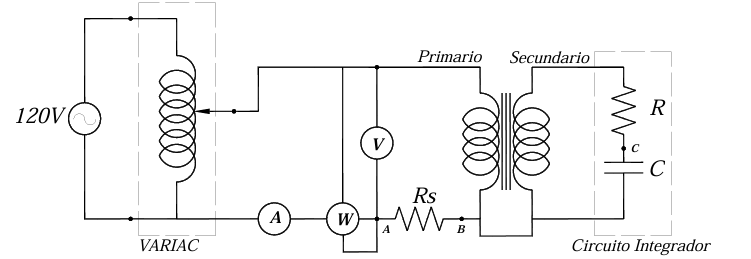
\includegraphics[width=\textwidth]{figures/figura-integrador.png}
\caption{Utilización del circuito integrador para la medición del ciclo de histéresis~\cite{guia}.}
\label{fig:integrador}
\end{figure}

\subsection{Núcleo macizo}
\begin{enumerate}
    \item Realizar el montaje con un núcleo macizo, tomando en cuenta que la constante de tiempo $RC$ debe ser muy superior al periodo de la red (por ejemplo, $C = \SI{1}{\micro\farad}$ y $R = \SI{150}{\kilo\ohm}$), utilizando las bobinas disponibles en el laboratorio. El circuito integrador está disponible en el laboratorio.
    \item Observar la forma de onda de la tensión y la corriente de alimentación.
    \item Discutir en torno a la forma de onda de la corriente.
    \item Medir la potencia consumida por la bobina.
    \item Trazar sobre papel milimetrado el ciclo de histéresis para una tensión de alimentación comprendida entre \SI{40}{V} y \SI{110}{V}.
    \item Calcular las escalas del ciclo de histéresis en unidades de campo (factor de escala vertical $K_v$ y factor de escala horizontal $K_h$, según las ecuaciones del marco teórico).
    \item Calcular:
          \begin{enumerate}
              \item Las pérdidas del núcleo.
              \item Las pérdidas por histéresis, a partir de las dimensiones del núcleo y el área del ciclo.
              \item Las pérdidas por corrientes parásitas (Foucault).
          \end{enumerate}
    \item Deducir el valor de la corriente de magnetización a la tensión especificada en el paso~5 y compararla con la corriente medida en el osciloscopio.
\end{enumerate}

\subsection{Núcleo laminado}
\begin{enumerate}
    \item Realizar el montaje con un núcleo laminado, tomando en cuenta una constante de tiempo $RC$ muy superior al periodo de la red (por ejemplo, $C = \SI{1}{\micro\farad}$ y $R = \SI{150}{\kilo\ohm}$), utilizando las bobinas disponibles en el laboratorio.
    \item Observar las formas de onda de la tensión de alimentación, la corriente y la inducción en el hierro.
    \item Discutir en torno a la forma de onda de la corriente.
    \item Medir la potencia consumida por la bobina.
    \item Trazar sobre papel milimetrado el ciclo de histéresis para una tensión de alimentación comprendida entre \SI{40}{V} y \SI{120}{V}.
    \item Calcular las escalas del ciclo de histéresis en unidades de campo.
    \item Calcular:
          \begin{enumerate}
              \item Las pérdidas del núcleo.
              \item Las pérdidas por histéresis, a partir de las dimensiones del núcleo y el área del ciclo.
              \item Las pérdidas por corrientes parásitas (Foucault).
          \end{enumerate}
    \item Deducir el valor de la corriente de magnetización a la tensión especificada en el paso~5 y compararla con la corriente medida en el osciloscopio.
\end{enumerate}

\begin{center}
    \textbf{Nota:} Para calcular la sección efectiva del circuito magnético con núcleo laminado, suponer un factor de apilamiento del \SI{93}{\percent}.
\end{center}
